\documentclass[journal]{IEEEtran}
\usepackage{amsmath,amsfonts}
\usepackage{algorithmic}
\usepackage{algorithm}
\usepackage[caption=false,font=normalsize,labelfont=sf,textfont=sf]{subfig}
\usepackage{textcomp}
\usepackage{stfloats}
\usepackage{url}
\usepackage{hyperref}
\usepackage{listings}
\usepackage{xcolor}
\usepackage{graphicx}
\usepackage{booktabs,threeparttable}
\hyphenation{op-tical net-works semi-conduc-tor IEEE-Xplore}
\usepackage{biblatex}
\addbibresource{references.bib}


% Syntax highlighting
\definecolor{codegreen}{rgb}{0,0.6,0}
\definecolor{codegray}{rgb}{0.5,0.5,0.5}
\definecolor{codepurple}{rgb}{0.58,0,0.82}
\definecolor{codeorange}{rgb}{0.9,0.45,0.3}
\definecolor{backcolour}{rgb}{0.95,0.95,0.92}
\lstdefinestyle{PythonStyle}{  
    language=Python, % Identifiers from C
	alsoletter={\{,\}},
    commentstyle=\color{codegreen}, % Green comments, like we used to
    keywordstyle=\color{blue}, % Blue keywords like 'int'
    numberstyle=\tiny\color{codegray}, % Grey numbers
    numbers=left, % Line number on left side 
    stringstyle=\color{codeorange}, % Strings look orange
    basicstyle=\ttfamily\footnotesize, % Same size for code as footnotes
    captionpos=t, % Caption on top
    xleftmargin=2em, % Margin on left side
    showstringspaces=false, % Don't show whitespaces
    tabsize=4, % Who doesn't use tabsize=4?
	emph=[1]{auto,break,case,char,const,continue,default,do, double, else, enum, extern, float, for, goto, if, int, long, register, return, short, signed, sizeof, static, struct, switch, typedef, union, unsigned, void, volatile, while, \{,\}},
    emphstyle=[1]{\color{codepurple}}, % Color keywords purple
    frame=lines, % Put the snippet within horizontal lines
}


\pagestyle{headings}
\begin{document}

\title{Assignment 3\\ INF-1400}

\author{Benjamin Aaboe Mjaatvedt\\ JustTemmie(change later)}
\markboth{INF-1400 Assignment 1 \today}%
{Mayhem}


\maketitle

\section{Introduction} \label{Section:Introduction}
In this program we were tasked with recreating the old game Mayhem. We instead wanted a challenge and made it 3D and with online multiplayer, and this of course posed some challenges.
\section{Design}\label{Section:Design}
As we wanted a 3D game, we ended up with not using Pygame, and instead used a library called Pyglet, and made our own game engine on top of it\footnote{Since this was not a part of the assignment, its design will not be discussed in this report.}.

Our engine provides some important super classes, some of these are Entity2D/3D and Game. Everything drawn or rendered to the screen is a subclass of Entity. All initiated, and visible Entities will be drawn/rendered to the screen. 

Mayhem needs: bullets, 2 players, some obstacles and pickups.

The 2 players has a lot of common attributes, but different methods, so we ended up with having a parent class "Player" who inherits from "Entity3D", and 2 child classes: "LocalPlayer" and "RemotePlayer" who inherits from "Player".

"Obstacle" and "Pickup" are parent classes, who are inherited by "Planet" and "Battery" respectively. These are also rendered to the screen so "Obstacle" and "Pickup" inherits from "Entity3D"

Since we wanted an online multiplayer game, we needed a Network class as well. This class is provided by our engine, so we only needed a method to handle the new requests.

The game itself is handled by the "Mayhem" class which is a subclass of the "Game" class. The "Game" class is the class that is responsible for rendering and update the game. Game updates and rendering are completely separate, they each got their own thread. This is done to get better performance.

The "Mayhem" class is also responsible for sending and checking network updates. This is done every game update.
\section{Challenges}\label{Section:Challenges}
\subsection{2D and 3D rendering}
One significant challenge we faced was managing the camera system effectively. Implementing a camera that can switch between different views—such as world rendering and HUD rendering requires careful handling of transformations and projections.
Ensuring that the camera correctly interprets the player's orientation and position in 3D space, particularly when dealing with upside-down scenarios.

In addition to the complexities of the camera system, optimizing rendering performance was another critical focus. Batched rendering was very important, by grouping similar entities together and rendering them in a single batch we save a ton of system overhead by minimizing the number of draw calls made to the GPU.

\subsection{Movement}
Implementing the player movement in a 3D environment presented significant challenges due to the complexity of the underlying maths. Initially, we were uncertain what the best way to control the player would be, but we ultimately decided to use the mouse cursor as a "digital joystick". This approach was heavily inspired by other games in the genre, particularly Elite Dangerous.

The final system allows the player's ship to rotate toward the mouse cursor. By employing some mathmatical calculations, we can accurately determine the direction the ship is facing based on its rotation, which is used in the process of generating thrust.

\subsection{Networking}
Since we wanted the game to be able to play online multiplayer, we had to code network code.
We decided to have a server that the clients has to connect to using UDP. The server works by taking in a packet from a client and then redistribute it to all the other clients. The server is also responsible for giving each client a unique ID.

The packet consists of the clients position, velocity, acceleration, rotation, if it has shoot that tick and if it died that tick. With this each client can update the remote players.

This is not the best solution. For example, if there is packet loss while you shoot, which can happen with UDP, the other players will not know about the bullet.
\subsection{Collision detection}
In 3D there is no easy way to do proper collision detection, and pyglet had no module to help with that. We were therefore forced to make our own collision detection system, and we did this by using the Gilbert-Johnson-Keerthi algorithm. 

The Gilbert-Johnson-Keerthi or GJK for short, works by calculating three points in the Minkowski difference to make a triangle and then check if it contains origin.~\cite{wikipediaGilbertJohnsonKeerthiDistance}

The Minkowski difference is just every point in one shape minus every point in another shape.~\cite{wikipediaMinkowskiAddition}

There is more to the algorithm than described above, for further reading~\cite{wikipediaGilbertJohnsonKeerthiDistance}.
\section{Discussion}\label{Section:Discussion}
The networking code is maybe a little to simple. All entities are handled client side, so you can hit two players with the same bullet, or two players can pick up the same battery pack.

One bottleneck is the collision detection. If there is more than 100, depends on the computer, hitboxes, the frame rate will drop significantly. If you look at the cProfile screenshot~[figure:\ref{fig:cprofile}] you can see that Hitbox3D furthest point takes up lot of time, so this function could probably be done better.

Another bottleneck is that we made the game in python. Python is not meant to make 3D games, or anything that needs performance for that matter. If we were to do it again, we would probably have chosen something like C++.

\begin{figure}[ht]
	\centering
	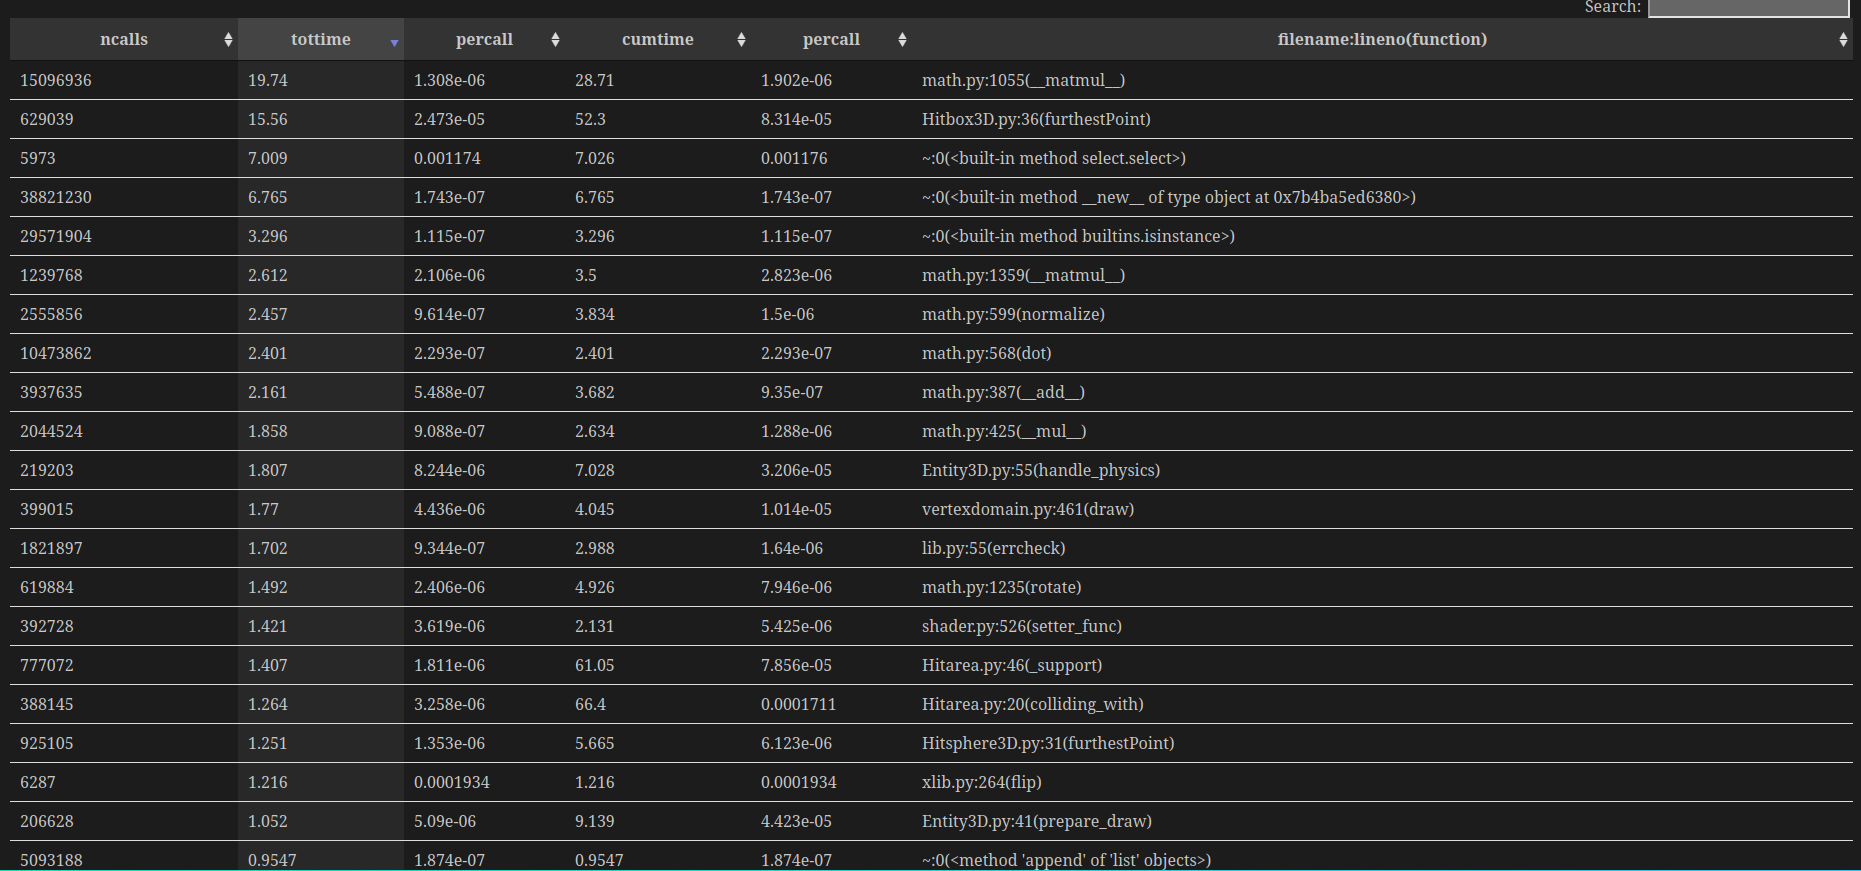
\includegraphics[width=\textwidth]{figures/cProfile.png}
	\caption{Screenshot of a part of the cProfile results}\label{fig:cprofile}
\end{figure}


\section{Conclusion}\label{Section:Conclusion}
\printbibliography{


\end{document}
